\documentclass[12pt]{article}

\usepackage{amsmath}
\usepackage{amssymb}
\usepackage{amsthm}
\usepackage{fullpage}
\usepackage{makecell}
\usepackage{tabularx}

\usepackage[dvipsnames]{xcolor}
\usepackage{tikz,tkz-euclide}
\usetikzlibrary{decorations.pathreplacing}
\usetikzlibrary{quotes,angles,calc,intersections}

\usepackage{titling}
\usepackage{pdfpages}
\usepackage{color}
\usepackage{hyperref}

\usepackage{common}
\usepackage{linear}

\begin{document}

\title{Vector Calculus Notes}
\author{Brendan Burkhart}
\maketitle

\tableofcontents
\newpage

\section{Orthogonal Projection}

\begin{figure}[ht!]
    \centering
    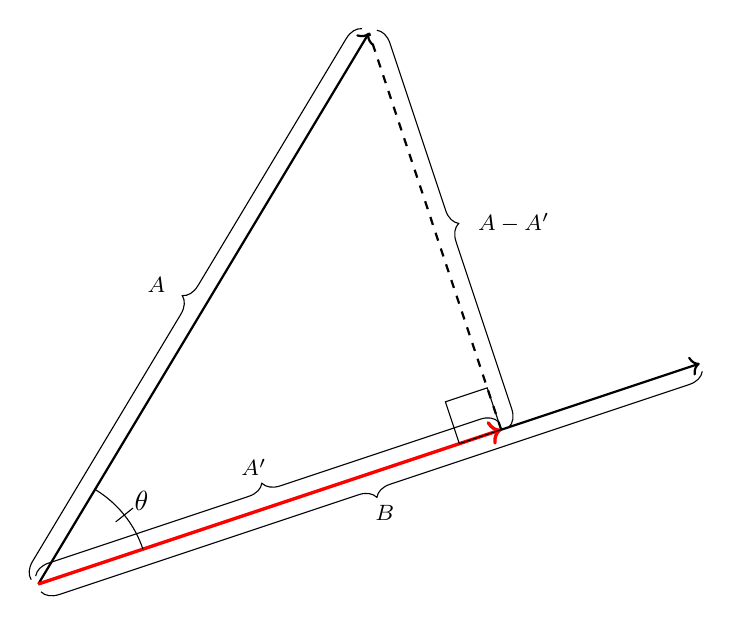
\begin{tikzpicture}[scale=1.4]
        \coordinate (O) at (0, 0);
        \coordinate (A) at (3, 5);
        \coordinate (B) at (6, 2);
        \coordinate (A') at ($(O)!(A)!(B)$);

        \draw [thick, ->] (O) -- (A);
        \draw [thick, ->] (O) -- (B);
        \draw [thick, dashed] (A') -- (A);
        \draw [very thick, red, ->] (O) -- (A');

        \draw [decorate,decoration={brace,amplitude=6pt,raise=3pt]}]
            (O) -- (A) node [black,midway,xshift=-0.6cm,yshift=0.3cm]
            {\footnotesize $A$};

        \draw [decorate,decoration={brace,amplitude=6pt,raise=3pt]}]
            (B) -- (O) node [black,midway,xshift=0.2cm,yshift=-0.5cm]
            {\footnotesize $B$};

        \draw [decorate,decoration={brace,amplitude=6pt,raise=3pt]}]
            (A) -- (A') node [black,midway,xshift=1.0cm, yshift=0.1cm]
            {\footnotesize $A - A'$};

        \draw [decorate,decoration={brace,amplitude=6pt,raise=3pt]}]
            (O) -- (A') node [black,midway,xshift=-0.2cm, yshift=0.5cm]
            {\footnotesize $A'$};

        \tkzMarkAngle[size=1cm,mark=|](B,O,A)
        \tkzLabelAngle[pos=1.2](B,O,A) {$\theta$}

        \tkzMarkRightAngle[size=0.4](A,A',O)
    \end{tikzpicture}
\caption{Orthogonal projection of $\vec{A}$ onto $\vec{B}$}
\label{fig:orthogonal-projection}
\end{figure}

Figure \ref{fig:orthogonal-projection} shows $A'$, the orthogonal projection of vector $A$ onto $B$. $\norm{A'}$ is the shortest distance between the head of $A$ and $B$.

\begin{thm} Let $A$ and $B$ be vectors. If $\theta$ is the angle between $A$ and $B$, and $A'$ is the orthogonal projection on $A$ onto $B$, then:
    \begin{itemize}
        \item $\cos\theta = \frac{A \cdot B}{\norm{A}\norm{B}}$
        \item $A' = \frac{A \cdot B}{B \cdot B}B$
    \end{itemize}
\end{thm}

\begin{proof}\proofbreak
    Let $C = A - B$. Then $C \cdot C = (A - B) \cdot (A - B)$, which can we expand to get $A \cdot (A - B) - B \cdot (A - B) = A \cdot A + B \cdot B - 2(A \cdot B)$. Therefore, $\norm{C}^2 = \norm{A}^2 + \norm{B}^2 - 2(A \cdot B)$. By the Law of Cosines, $A \cdot B = \norm{A}\norm{B}\cos\theta$, so $\cos\theta = \frac{A \cdot B}{\norm{A}\norm{B}}$.

    Let $d \in \R$ such that $C = dB$. Then since $(A - dB) \cdot B = 0$, we know $A \cdot B - dB \cdot B = 0$, so $A \cdot B = d(B \cdot B)$. This implies that $d = \frac{A \cdot B}{B \cdot B}$. Since $C = dB$, we then have $C = \frac{A \cdot B}{B \cdot B}B$.
\end{proof}

\end{document}
